\section{Appendix}
Hier werden die extra Content abgebildet.

\subsection{Ältere Versionen des Komponentendiagramms}


\begin{figure}[!hbt]
    \centering
    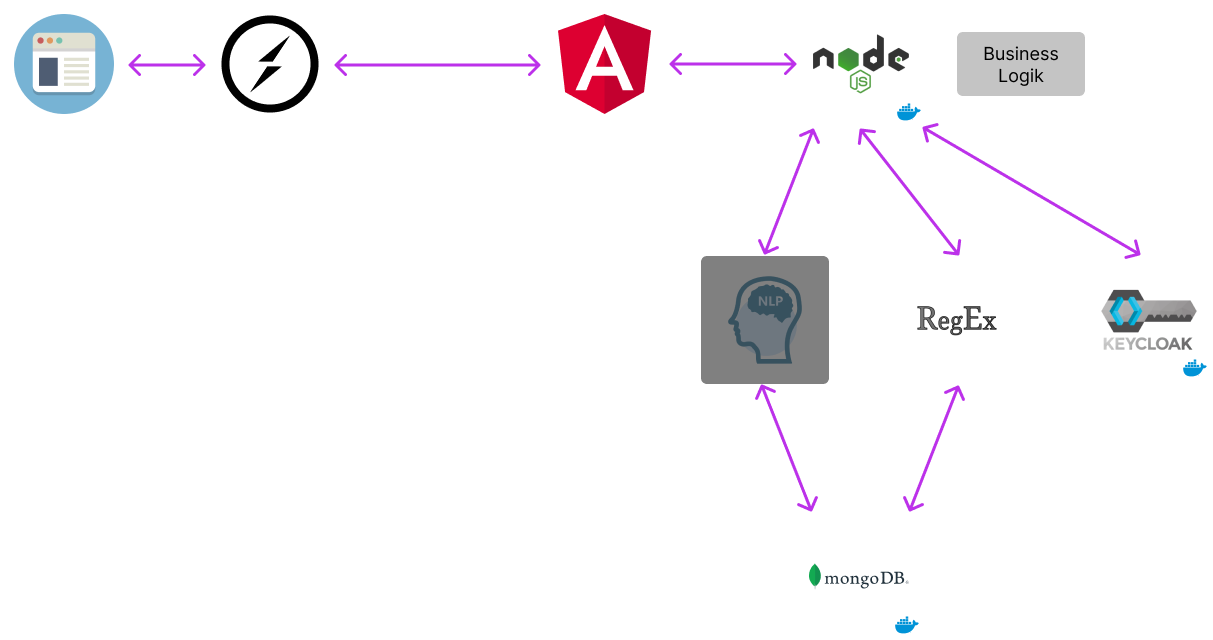
\includegraphics[width=1.0\textwidth]{bilder/technologien/Komponenten-Diagram-v1.png}
    \caption{Komponentendiagramm v1.0}
    \label{fig:Komponentendiagramm_v1.0}
    \end{figure}

\noindent In dieser Version haben wir erst einmal die Struktur von unseren Komponentengesucht und eine
grobe Darstellung erstellt. Was wir hier aber nicht wussten ist, wie wir das NLP darstellen sollten.
NLP war für uns vorher eine optionale Möglichkeit.

    \begin{figure}[!hbt]
        \centering
        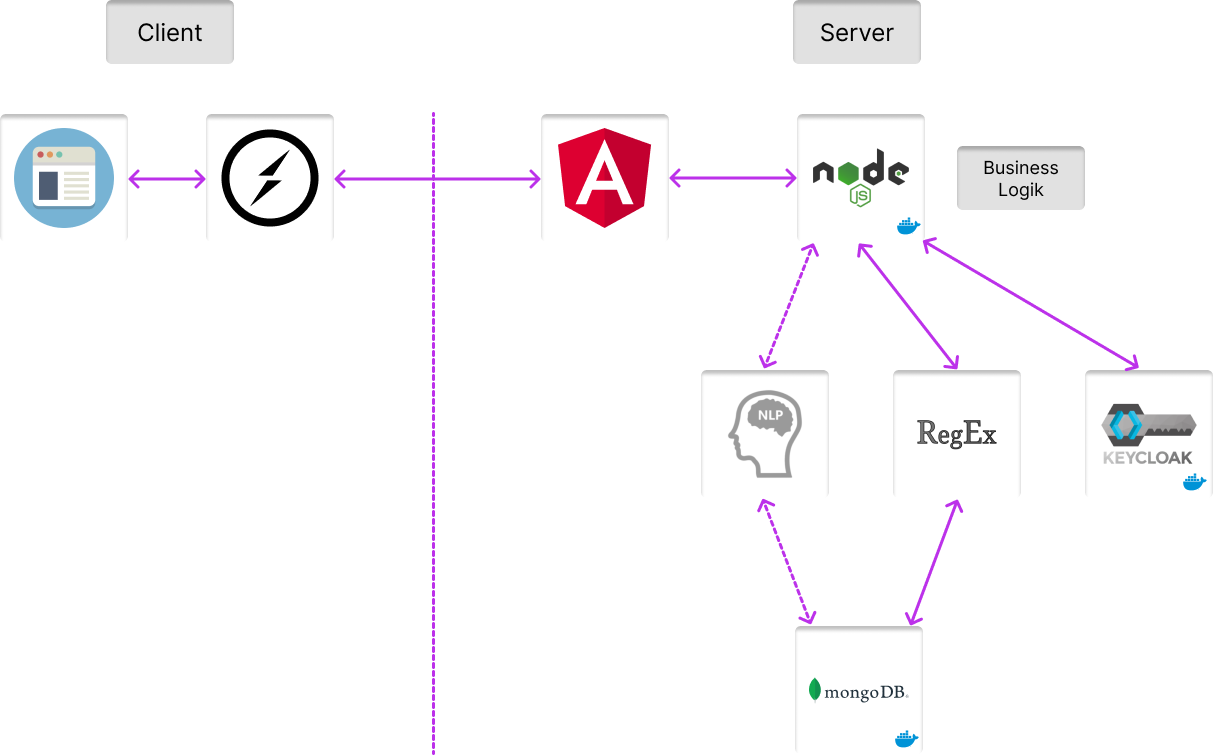
\includegraphics[width=1.0\textwidth]{bilder/technologien/Komponentendiagram v1.1.png}
        \caption{Komponentendiagramm v1.1}
        \label{fig:Komponentendiagramm_v1.1}
        \end{figure}
        \FloatBarrier % prevent pictures from appearing under a different section

\noindent In dieser Darstellung haben wir die einzelnen Komponenten in Server und Client 
eingeteilt, um die Struktur besser zu verstehen. Wir haben aber die Abtrennung nicht richtig anzeigen können
und das NLP haben wir auch nicht klar als optional zeigen können.
        